% SPDX-License-Identifier: CC-BY-SA-4.0
% Author: Matthieu Perrin
% Part: 
% Section: 
% Sub-section: 
% Frame: 

\begingroup

\begin{frame}{Arbre de dérivation }

  Soit \alert{$G = \langle \Sigma, \Gamma, S, R \rangle$} une grammaire algébrique.

  \begin{block}{Arbre de dérivation (ou arbre de la syntaxe concrète, CST)}

    Chaque génération de $G$ peut être représentée par un arbre.

    \begin{description}
    \item[Racine :] l'axiome $S$\\
    \item[N\oe ud interne :] Symbole non-terminal de $\Gamma$
    \item[Feuille :] Symbole terminal de $\Sigma$, ou $\varepsilon$ ($\varepsilon$ ne peut pas avoir de frère)
    \item[Filiation :] Si les fils de $A$ sont $a_1$, ..., $a_n$, alors $A \rightarrow a_1...a_n \in R$
    \end{description}
    Le mot généré est alors la concaténation des feuilles de l'arbre.
  \end{block}



  \begin{exampleblock}{Exemple}

    \vspace{-5mm}
    \begin{minipage}{.8\textwidth}
      \example{$G = \left\langle \{a, b, c\}, \{S, B\}, S, \left\{\begin{array}{rcl} S &\rightarrow & aSb \,|\, B \\ B &\rightarrow & cB \,|\, \varepsilon \end{array}\right\} \right\rangle$}.\\

      \vspace{2mm}
      Arbre de la syntaxe concrète de $aacbb$ :
    \end{minipage}%
    \begin{minipage}{.2\textwidth}
      \vspace{-2mm}
      \scalebox{.9}{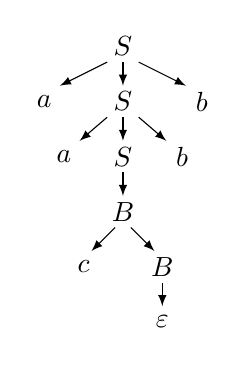
\begin{tikzpicture}
          \draw(5.00,5.0) node{$S$};
          \draw(4.00,4.3) node{$a$};
          \draw(5.00,4.3) node{$S$};
          \draw(6.00,4.3) node{$b$};
          \draw(4.25,3.6) node{$a$};
          \draw(5.00,3.6) node{$S$};
          \draw(5.75,3.6) node{$b$};
          \draw(5.00,2.9) node{$B$};
          \draw(4.50,2.2) node{$c$};
          \draw(5.50,2.2) node{$B$};
          \draw(5.50,1.5) node{$\varepsilon$};

          \draw[-latex] (4.80,4.8) -- (4.20,4.5);
          \draw[-latex] (5.00,4.8) -- (5.00,4.5);
          \draw[-latex] (5.20,4.8) -- (5.80,4.5);

          \draw[-latex] (4.80,4.1) -- (4.45,3.8);
          \draw[-latex] (5.00,4.1) -- (5.00,3.8);
          \draw[-latex] (5.20,4.1) -- (5.55,3.8);

          \draw[-latex] (5.00,3.4) -- (5.00,3.1);

          \draw[-latex] (4.90,2.7) -- (4.60,2.4);
          \draw[-latex] (5.10,2.7) -- (5.40,2.4);

          \draw[-latex] (5.50,2.0) -- (5.50,1.7);

      \end{tikzpicture}}
    \end{minipage}%

  \end{exampleblock}
\end{frame}

\endgroup
